%
\documentclass{beamer}
\usepackage{caption}
\usepackage{subcaption}
\usepackage{pdfpages}
\usepackage{graphicx}
\usepackage{../../arbenson-math}

\usetheme{boxes}
\usecolortheme{seahorse}

\AtBeginSection[]
{
  \begin{frame}<beamer>
    \frametitle{\thesection}
    \tableofcontents[currentsection]
  \end{frame}
}

\title{CME 193: Introduction to Scientific Python \\
Lecture 5: Data Visualization \& Web Scraping}
\author{
Dan Frank \\
\vspace{0.1in}
Institute for Computational and Mathematical Engineering (ICME)}
\date{January 23, 2014}
\begin{document}

\maketitle

\begin{frame}
\frametitle{Administrivia}
\begin{itemize} 
\setlength{\itemsep}{0.1in}
\item{HW 4 due next class }
\item{No HW 5}
\item{Austin Benson will teach guest lecture}
\end{itemize}
\end{frame}




\section{IDEs, Debugging, Version Control, etc.} 

\begin{frame}
\frametitle{Debugging: General Principles}
How do I make my code bug free?
\begin{enumerate}
\item First, don't write bugs! (e.g. informative variable/function names, encapsulation, etc.)
\item Isolate the problem: module $\Rightarrow$ function $\Rightarrow$ variable
\item Be able to consistently reproduce the problem
\item Read the error messagees
\item print statements  
\item Explore the code interactively with a debugger
\end{enumerate}
\end{frame}

\begin{frame}
\frametitle{Debugging}
I've written a function or script and it's giving me a weird error... now what?
\codeblock{code/debug.py}
\end{frame}

\begin{frame}
\frametitle{Debugging: ipdb}
What can I do within the debugger?
\begin{enumerate}
\item n (next)
\item ENTER (repeat previous)
\item q (quit)
\item p \texttt{variable} (print value)
\item c (continue)
\item l (list where you are)
\item s (step into subroutine)
\item r (continue till the end of the subroutine)
\item plus anything you can normally do at a python terminal
\end{enumerate}
\end{frame}

\begin{frame}
\frametitle{Debugging: ipdb}
\begin{figure}[h]
\centering
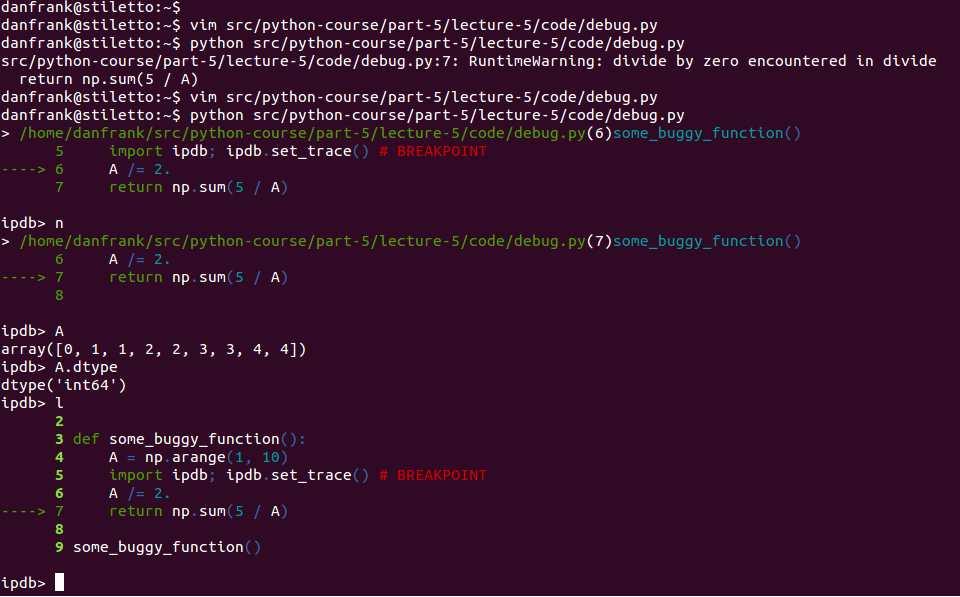
\includegraphics[width=.9\textwidth]{images/debug.png}
\end{figure}
\end{frame}



% we should probably have talked about this before
\begin{frame}
\frametitle{IDEs}
Not all software engineers use them but Integrated Development Environments can be very helpful in developing code. Functionality may include
\begin{itemize}
\setlength{\itemsep}{0.1in}
\item{source code editor with syntax highlighting}
\item{autocompletion and goto definitions}
\item{debugging}
\item{integration with terminal}
\end{itemize}
No standard IDE for Python, but eclipse, emacs, vim, etc. can be configured. Each coder has their own setup. iPython provides many of these functions within a terminal.
\end{frame}

\begin{frame}
\frametitle{Version Control}
Version control enables different people working on the same code base to coordinate their efforts.
\begin{itemize}
\setlength{\itemsep}{0.1in}
\item{maintain history of code development}
\item{tracking differences between current versions and older versions}
\item{create branches of code so different features can be worked on simultaneously and merged together later}
\end{itemize}
There are many tools for version control but the standards are \textbf{subversion} and more recently \textbf{git}. This course is currently coordinated through \url{github.com}
\end{frame}

\section{Matplotlib}

\begin{frame}
\frametitle{What is Matplotlib?}

matplotlib.org: matplotlib is a python 2D plotting library which produces publication quality figures in a variety of hardcopy formats and interactive environments across platforms. matplotlib can be used in python scripts, the python and ipython shell (ala MATLAB or Mathematica), web application servers, and six graphical user interface toolkits.

\begin{itemize}
\setlength{\itemsep}{0.1in}
\item{matplotlib is the standard Python plotting library}
\item{We will prmarily be using \texttt{matplotlib.pyplot} for data analysis}
\item{Can create histograms, power spectra, bar charts, errorcharts, scatterplots, etc with a few lines of code}
\end{itemize}
\end{frame}

\begin{frame}
\frametitle{Scatter Plot}
\lstset{basicstyle=\scriptsize}
\codeblock{code/line_plot.py} 
\begin{figure}[h]
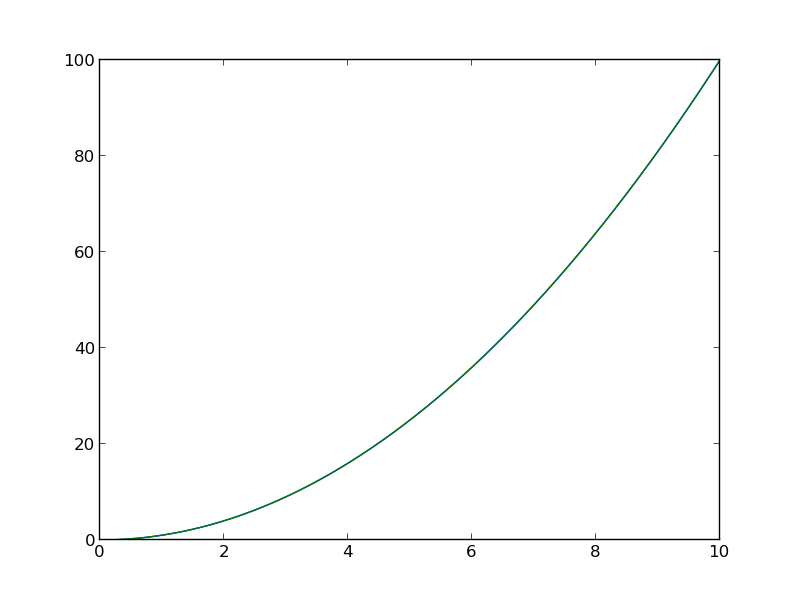
\includegraphics[width=.6\textwidth]{images/line_plot.png}
\end{figure}
\end{frame}

\begin{frame}
\frametitle{Scatter Plot+}
\begin{figure}[h]
\centering
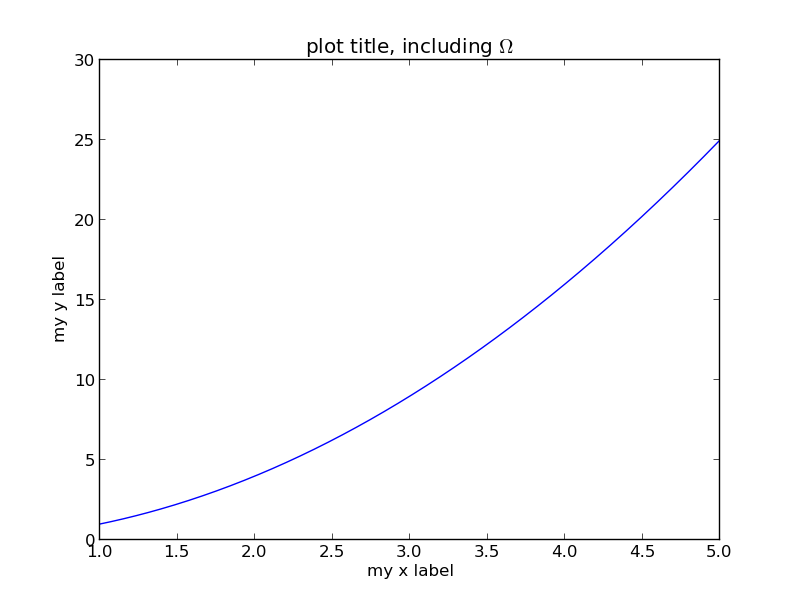
\includegraphics[width=.9\textwidth]{images/line_plot_plus.png}
\end{figure}
\end{frame}

\begin{frame}
Adding titles and labels
\frametitle{Scatter Plot+}
\codeblock{code/line_plot_plus.py}
\end{frame}

\begin{frame}
\frametitle{Scatter Plot++}
\begin{figure}[h]
\centering
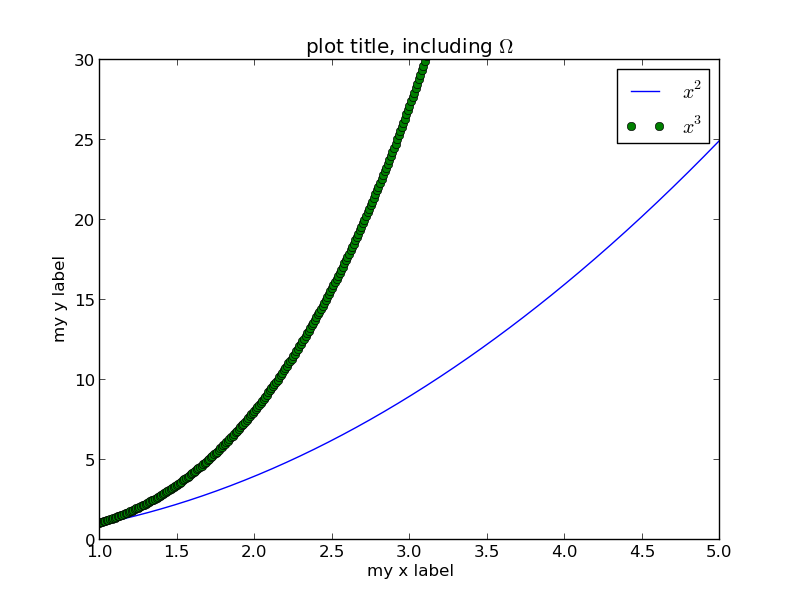
\includegraphics[width=.9\textwidth]{images/line_plot_plus2.png}
\end{figure}
\end{frame}

\begin{frame}
\frametitle{Scatter Plot++}
Adding multiple lines and a legend
\lstset{basicstyle=\small}
\codeblock{code/line_plot_plus2.py}
\end{frame}

\begin{frame}
\frametitle{Histogram}
\begin{figure}[h]
\centering
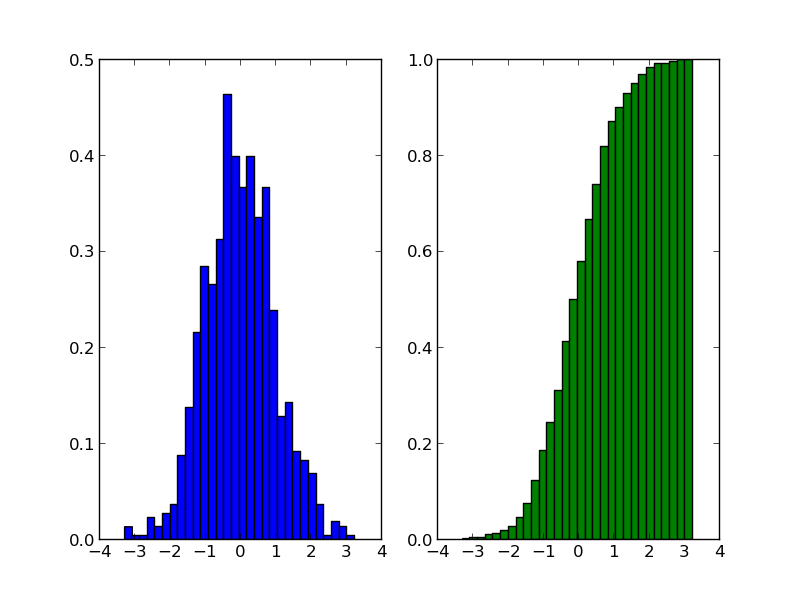
\includegraphics[width=.9\textwidth]{images/histogram.png}
\end{figure}
\end{frame}

\begin{frame}
\frametitle{Histogram}
\lstset{basicstyle=\small}
\codeblock{code/histogram.py}
\end{frame}


\begin{frame}
\frametitle{Box Plot}
\begin{figure}[h]
\centering
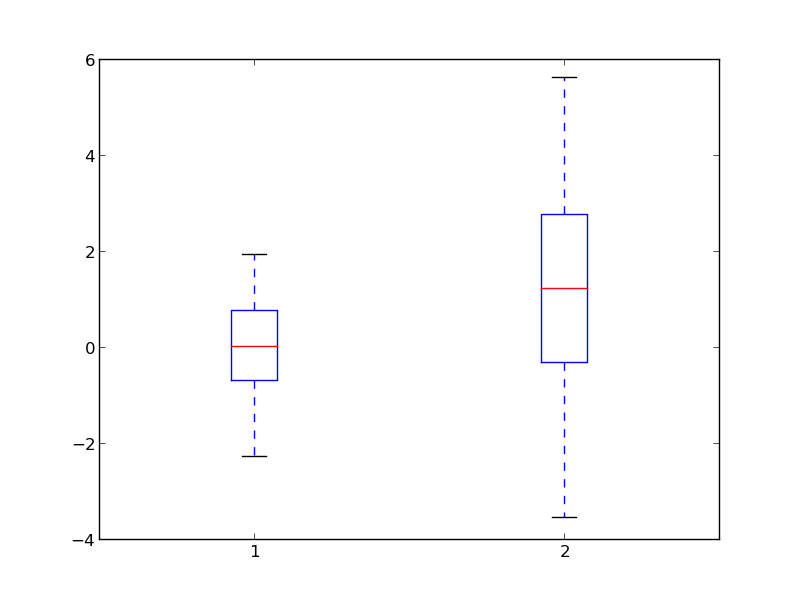
\includegraphics[width=.9\textwidth]{images/boxplot.png}
\end{figure}
\end{frame}

\begin{frame}
\frametitle{Box Plot}
\codeblock{code/boxplot.py}
\end{frame}


\begin{frame}
\frametitle{Scatter Plot Matrix}
\begin{figure}[h]
\centering
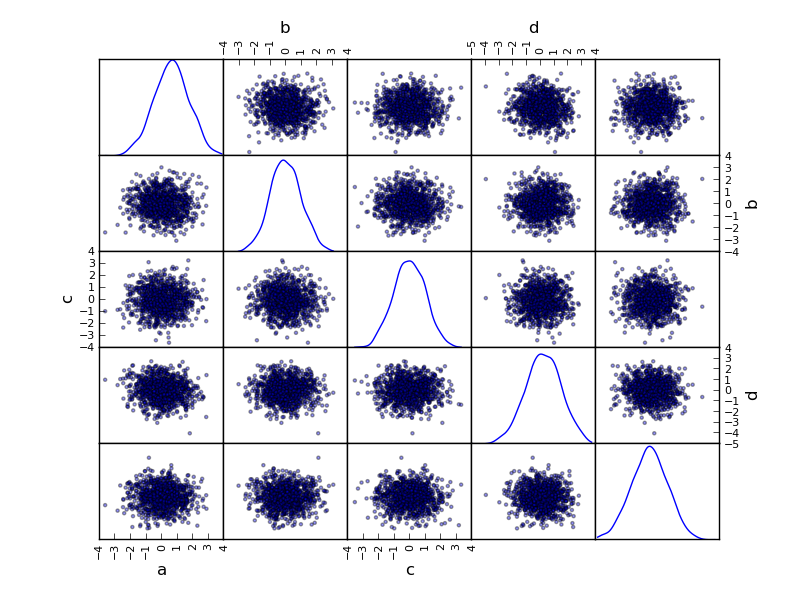
\includegraphics[width=.9\textwidth]{images/scattermatrix.png}
\end{figure}
\end{frame}


\begin{frame}
\frametitle{Scatter Plot Matrix}
\texttt{matplotlib} doesn't have everything, especially functions that are designed to act on more than one axis at once. 
\codeblock{code/scattermatrix.py}
\end{frame}

\begin{frame}
\frametitle{Image Plot}
\begin{figure}[h]
\centering
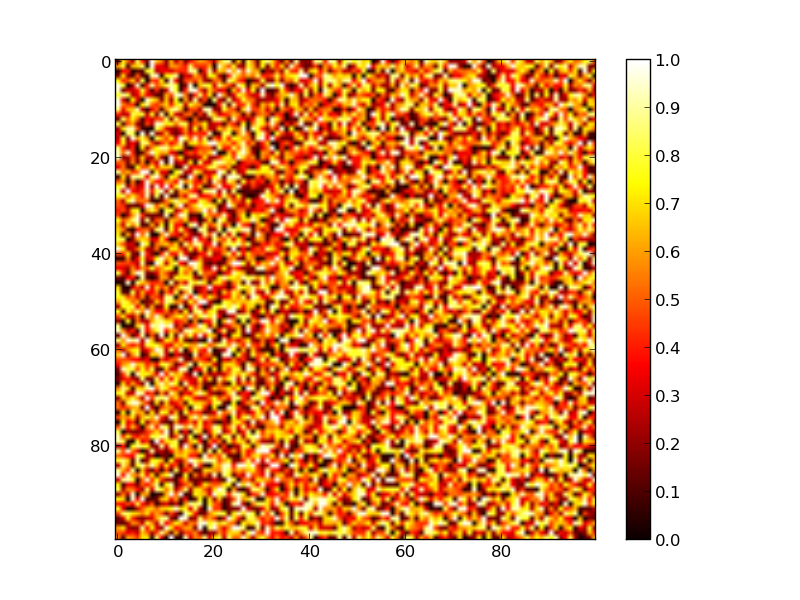
\includegraphics[width=.9\textwidth]{images/imageplot.png}
\end{figure}
\end{frame}


\begin{frame}
\frametitle{Image Plot}
\codeblock{code/imageplot.py}
\end{frame}

\begin{frame}
\frametitle{Wire Plot}
\begin{figure}[h]
\centering
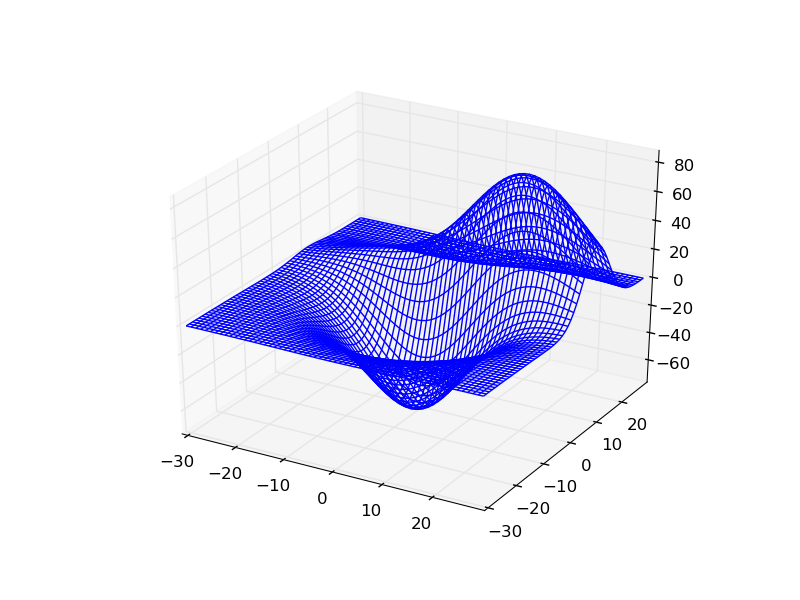
\includegraphics[width=.9\textwidth]{images/wire.png}
\end{figure}
\end{frame}

\begin{frame}
\frametitle{Wire Plot}
matplotlib toolkits extend funtionality for other kinds of visualization
\codeblock{code/wire.py}
\end{frame}

\section{Web Scraping}

\begin{frame}
\frametitle{Web Scraping Ingredients}
Webscraping HTML involves...
\vspace{0.2in}
\begin{itemize}
\setlength{\itemsep}{0.1in}
\item{visual inspection - \texttt{Chrome Developer Mode \& Firebug}}
\item{browser sessions and interacting with HTML - \texttt{mechanize}}
\item{HTML parsing/searching - \texttt{BeautifulSoup}}
\vspace{0.2in}

warning: javascript makes things tricky... check out \textit{selenium} if you need to interact with javascript
\end{itemize}
\end{frame}


\begin{frame}
\frametitle{Webscraping Example}
Want to verify that wikipedia's plot
\begin{figure}[h]
\centering
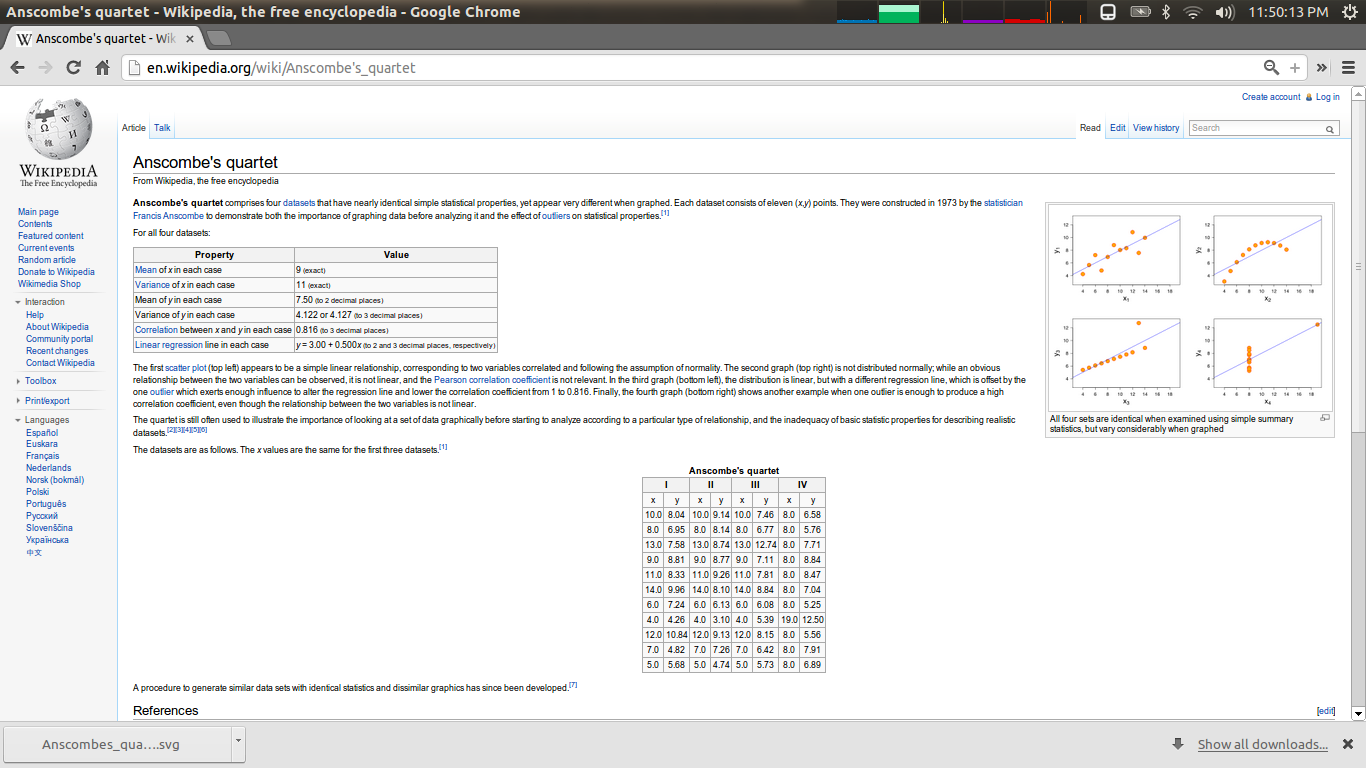
\includegraphics[width=.9\textwidth]{images/anscombe.png}
\end{figure}
\end{frame}

\begin{frame}
\frametitle{Webscraping Example}
Recreate the plot ourselves by scraping the data and plotting
\begin{figure}[h]
\centering
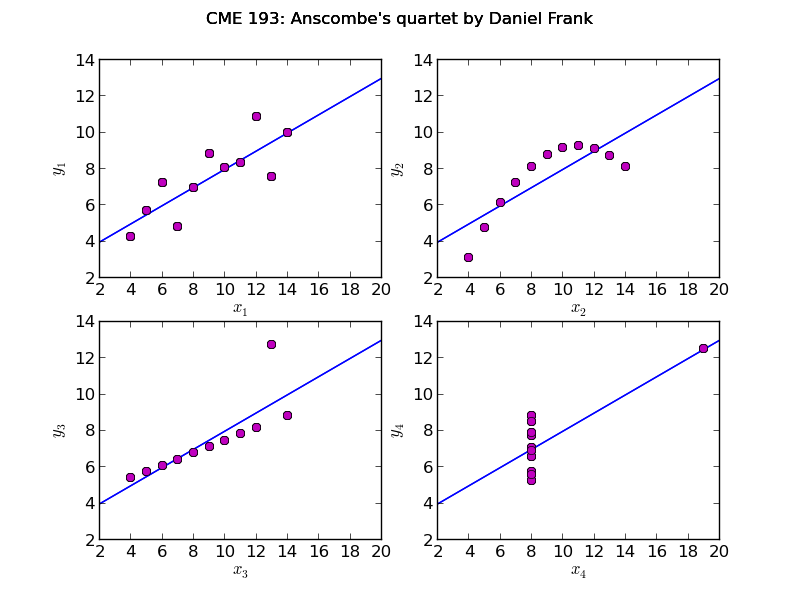
\includegraphics[width=.9\textwidth]{images/quartet.png}
\end{figure}
\end{frame}

\begin{frame}
\frametitle{Webscraping Example: Visual Inspection}
In Chrome Developer Mode we can use 'inspect element' to look at the HTML associated with the table we're interested in.

\begin{figure}[h]
\centering
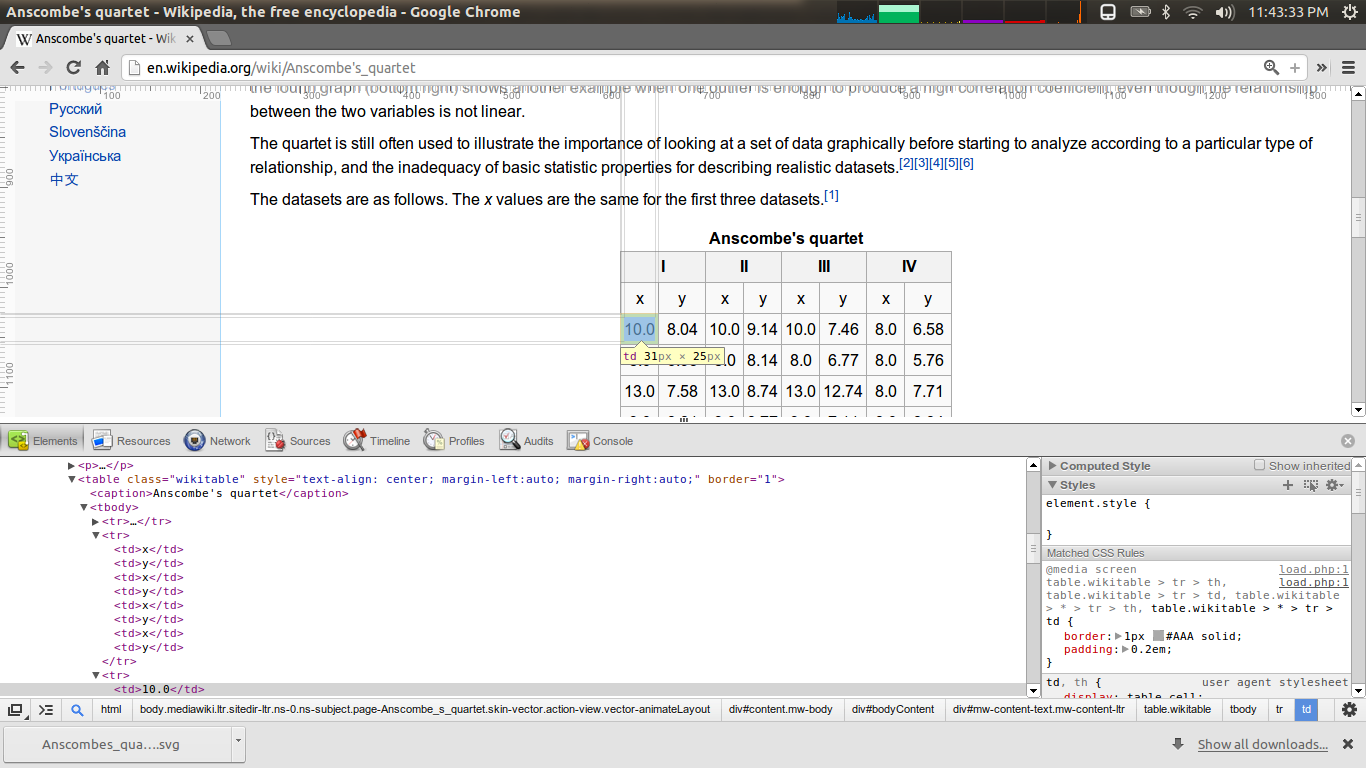
\includegraphics[width=.9\textwidth]{images/chrome_devel.png}
\end{figure}
\end{frame}


\begin{frame}
\frametitle{Webscraping Example: Visual Inspection}
\lstset{basicstyle=\tiny}
\codeblock{code/scrape.py}
\end{frame}

\end{document}


